\chapter{Results and Discussion}\label{ch:results}
\section{Reading the evidence}
The results are derived from the saved predictions, pair statistics, training records, export outputs and runtime profiles. All empirical tables and plots in this chapter are generated by \code{scripts/generate_artifacts.py}. The generation step records hashes of its input result files. Headline values in the prose use generated LaTeX macros so a rerun cannot silently leave those values inconsistent with the tables.

Three outcomes are kept separate throughout. Retrieval asks whether the correct identity appears in a ranked list. Correct verification asks whether the pipeline accepts the correct identity. Planar success additionally asks whether the accepted transformation agrees with an independent ground-truth homography. A result may satisfy one outcome without satisfying the next. This distinction is especially important for Tokyo, where no true planar or metric-pose error can be computed from the downloaded metadata.

\section{Oracle-pair local matching}
\resultinput{matching.tex}
\Cref{tab:matching} compares SIFT--FLANN and SuperPoint--LightGlue on identical positive image pairs with common geometry settings. Supplying the correct reference removes candidate-search failure from this comparison. The inlier statistics describe each method's own tentative matches, so a higher count is interpreted alongside acceptance and corner-error success rather than as a standalone proof of accuracy.

On the selected HPatches illumination pairs, SIFT achieves \HpIllumSift\% accepted five-pixel homography success, while the learned combination achieves \HpIllumLearned\%. This supports an illumination-robustness benefit on this subset. The result remains conditional on the selected scenes, resolution and verification policy. It does not show that every illumination condition is solved or that the matcher can reconstruct detail absent from an underexposed image.

On the viewpoint pairs, the success values are \HpViewSift\% for SIFT and \HpViewLearned\% for the learned combination. The learned method therefore does not dominate every geometric condition in the tested set. In particular, accepted estimates can still extrapolate poorly to reference corners outside the supported region. This observation cautions against using a greater number of matches as a substitute for evaluated alignment accuracy.

\begin{figure}[htbp]\centering
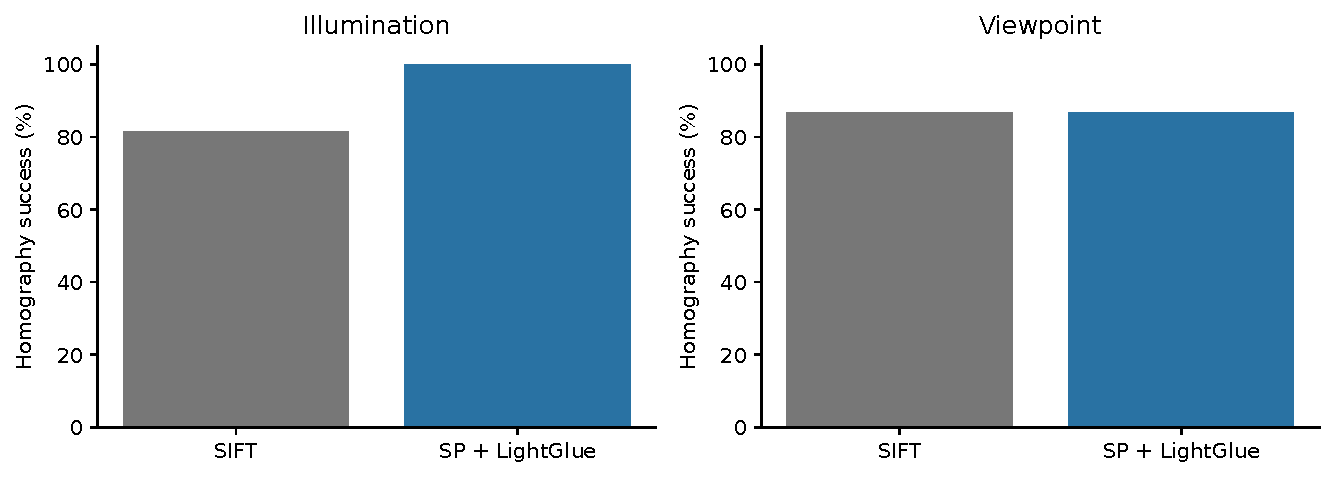
\includegraphics[width=\textwidth]{hpatches_success.pdf}
\caption{Measured oracle-pair homography success on the selected real HPatches sequences. A success requires accepted geometry and mean corner error no greater than five working pixels.}\label{fig:hpatches-success}
\end{figure}
\Cref{fig:hpatches-success} emphasises the different illumination and viewpoint outcomes. The illumination gain is consistent with the motivation for learned features, while the viewpoint result provides a negative control against an unconditional improvement claim. Different subsets or thresholds may change the comparison, and the artifact makes those choices explicit rather than treating its rates as universal model properties.

\ifFullReport
\begin{figure}[htbp]\centering
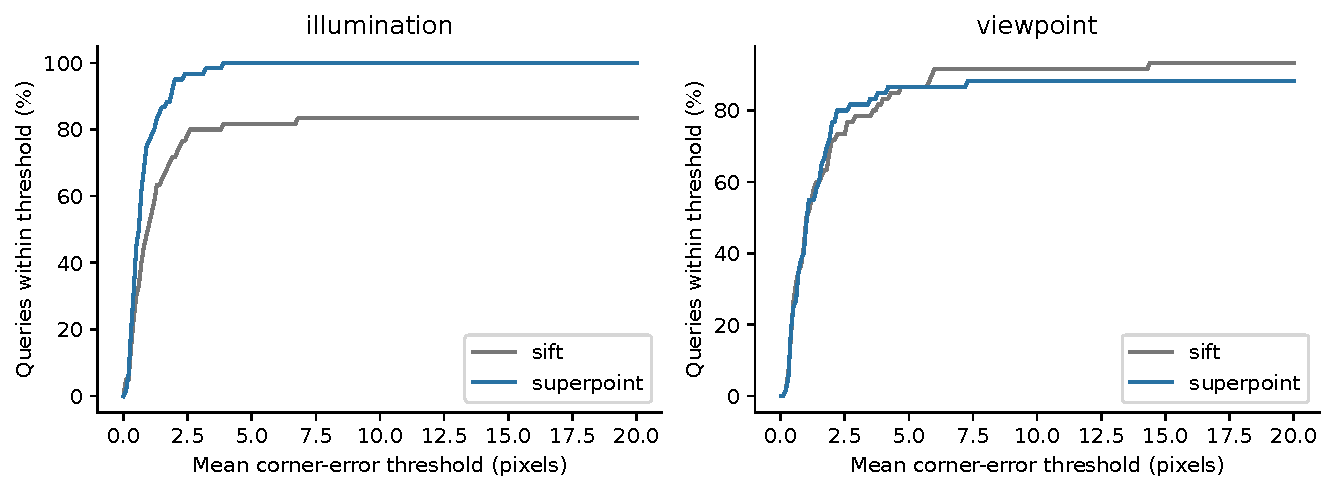
\includegraphics[width=\textwidth]{corner_ecdf.pdf}
\caption{Cumulative accepted-homography accuracy against corner-error threshold. Failed or rejected estimates remain outside the curve at finite thresholds; all pairs remain in each denominator.}\label{fig:corner-ecdf}
\end{figure}
\Cref{fig:corner-ecdf} provides more information than a single threshold. A method whose finite-error estimates are precise can still have a low maximum curve value because many pairs fail. Conversely, accepted estimates with large corner error contribute only at loose thresholds. Keeping failures in the denominator avoids presenting a conditional accuracy curve as if it represented all evaluated queries.
\fi

\section{Place retrieval on real Tokyo photographs}
\resultinput{retrieval_tokyo.tex}
\Cref{tab:retrieval-tokyo} gives the custom cross-time retrieval results. Day-to-night Recall@1 is \DayNightSiftRecall\% for exhaustive SIFT, \DayNightLearnedRecall\% for exhaustive learned local matching, and \DayNightGlobalRecall\% for CosPlace. The full hierarchy correctly verifies \DayNightFullVerified\% of those selected queries. The corresponding SIFT correctly verified-place rate is \NightSiftVerified\%, which is lower than its retrieval recall because some correct ranked candidates lack enough accepted local evidence.

The saturation of learned and global recall on this split is a property of the selected protocol. It uses aligned front-facing observations and a gallery of \TokyoSites{} selected sites. It does not use the official street-view database. Small-sample intervals and the task distinction are therefore necessary qualifications, not minor reporting details. Perfect observed recall in this setting cannot establish perfect recognition over a city or across arbitrary camera directions.

The daytime viewpoint-change result exposes a complementary weakness. CosPlace Recall@1 falls to \DayViewGlobalRecall\%, and the primary full pipeline correctly verifies \DayViewFullVerified\% of queries. Exhaustive SIFT correctly verifies \ViewSiftVerified\%, and exhaustive learned matching verifies \ViewLearnedVerified\%. The hierarchy therefore sacrifices some recoverable cases when its shortlist excludes a useful reference. This is a measured negative result for the chosen global stage and shortlist policy.

\begin{figure}[htbp]\centering
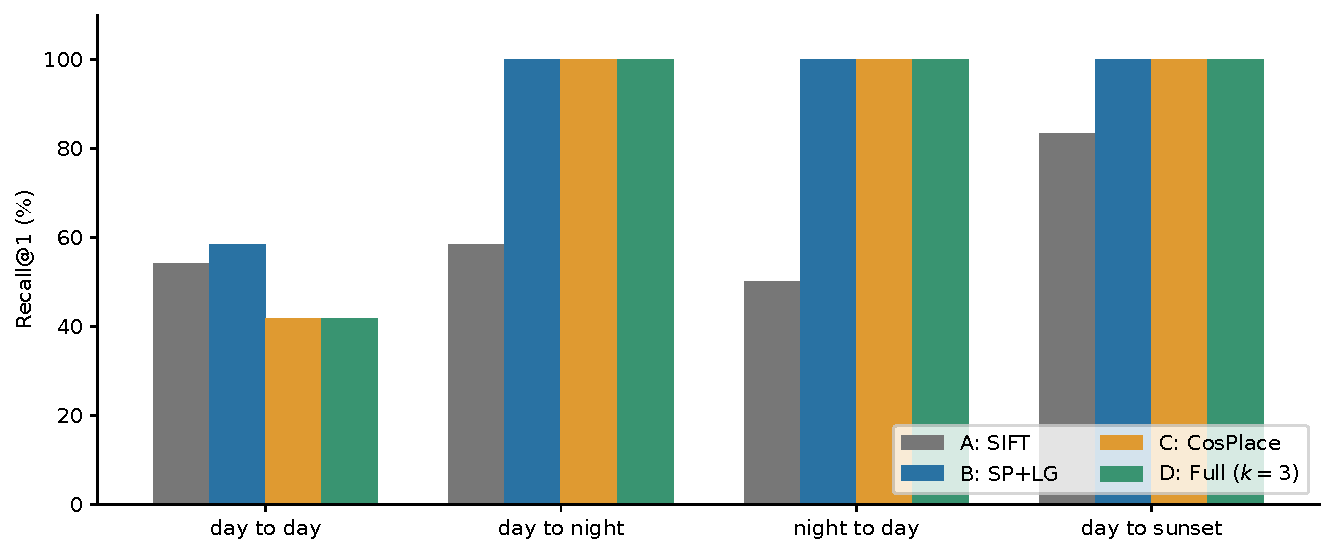
\includegraphics[width=\textwidth]{tokyo_retrieval.pdf}
\caption{Recall@1 on the actual selected Tokyo query photographs. Day-to-day uses a different labelled viewing direction; the other splits use the retained front-facing records across time.}\label{fig:tokyo-retrieval}
\end{figure}
\Cref{fig:tokyo-retrieval} shows that the split label alone does not determine difficulty. Appearance change with similar viewpoint can be easier than unchanged daylight with reduced overlap. This supports retaining both kinds of variation in future validation. It also suggests that collecting several reference directions may be more useful than adding another photometric variant of one view, although that proposed collection strategy has not been tested here.

Night-to-day and sunset results are reported separately in the table because descriptor extraction and matching are direction-sensitive. They should not be counted as independent additional cities or sites. Their shared identities and reference observations limit any claim about geographic generalisation. The evidence supports behaviour under the recorded cross-time pairings.

\section{HPatches retrieval and end-to-end planar success}
\resultinput{retrieval_hpatches.tex}
\Cref{tab:retrieval-hpatches} evaluates retrieval among the selected HPatches reference images. Its scene-identity labels are sequence labels, not geographic locations. The task is useful for checking whether a coarse descriptor identifies a plausible reference before geometric verification, but it remains a custom distractor gallery rather than a standard place-recognition leaderboard.

\resultinput{pipeline-geometry.tex}
\Cref{tab:pipeline-geometry} adds the complete planar-success criterion. A correctly selected identity may still fail the five-pixel condition. Likewise, good oracle-pair accuracy does not guarantee that the end-to-end system finds that reference. This table is the appropriate evidence when the claim concerns an accurately anchored planar post rather than recognition alone.

The comparison also illustrates a property of geometric verification: it can reject a correct place for application-valid reasons. A query may show a small region of the scene with insufficient spatial extent for stable extrapolation to the full reference plane. The appropriate response for the current renderer is to withhold the overlay, even though a broader semantic recogniser might confidently name the street. Future region-specific anchor evaluation could distinguish this case from complete recognition failure.

\section{Synthetic appearance stress tests}
\resultinput{retrieval_synthetic.tex}
\Cref{tab:retrieval-synthetic} reports the seeded transformations as their own collection. Learned methods retain strong source-image recognition under the implemented night stressors, while severe attenuation reduces SIFT's supported decisions. This is consistent with the implementation-level motivation, but the dependence on a small set of base images remains substantial.

Synthetic night retains the exact original scene content and applies a known warp. It cannot reproduce all changes in visibility, illumination direction, light-source placement or sensor response. The fog-like transformation likewise does not establish weather robustness. The actual input examples in \cref{fig:synthetic-data} define the scope of the claim more precisely than the condition names alone.

The three seeds vary random perturbations, not the physical scene population. Treating all generated frames as independent places would overstate evidence. For this reason, the report does not combine synthetic and real-night queries into one headline ``night robustness'' score. Such an aggregate would obscure both the shared-source dependence and the different ground-truth availability.

\section{Stage ablations}
\resultinput{ablations.tex}
\Cref{tab:ablations} compares candidate limits and stage removal. Exhaustive learned matching provides the no-global-stage reference. Increasing the shortlist permits more comparisons but does not guarantee more correct accepted places: additional candidates can also create competing or incorrect geometric hypotheses. The measured viewpoint split shows that candidate recall and local support must be considered jointly.

\begin{figure}[htbp]\centering
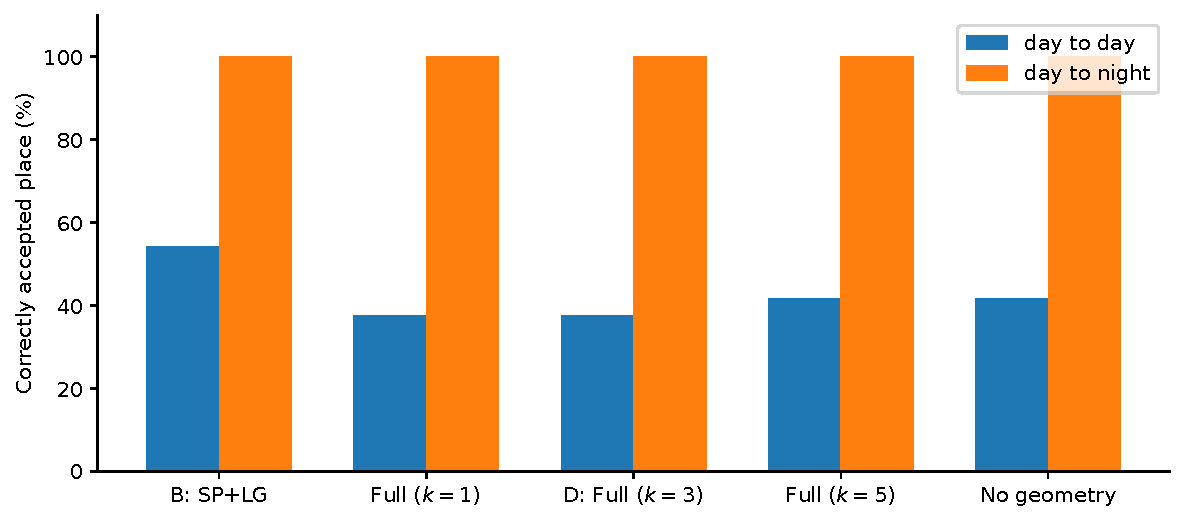
\includegraphics[width=\textwidth]{stage_ablation.pdf}
\caption{Measured correctly accepted-place rates for retrieval and geometry ablations. ``No geometry'' is a diagnostic acceptance policy without an anchored transform.}\label{fig:ablation}
\end{figure}
\Cref{fig:ablation} makes the hierarchy's main trade-off visible. When the global representation already places the correct reference near the top, a small shortlist retains the observed success of exhaustive learned matching. When viewpoint changes move the useful reference down the ranking, exhaustive search can recover cases missed by the primary hierarchy. The runtime comparison in \cref{ch:deployment} quantifies the cost of that additional search.

\subsection{Unknown places and false acceptance}
\resultinput{open-set.tex}
\Cref{tab:open-set} reports the unknown-query diagnostic. It is possible for learned local matching to accept a geometrically plausible wrong candidate even when the image collection is disjoint. Increasing the candidate count exposes more such opportunities. A no-geometry policy necessarily accepts a top-ranked candidate for every unknown query in this implementation.

These failures matter for social AR because a false acceptance can display a post at the wrong physical location. The small diagnostic cannot establish a production false-positive bound, particularly for nearby look-alike buildings or adversarial replay. It does demonstrate why retrieval similarity and homography support cannot be treated as complete identity assurance. The discussion of abuse in \cref{ch:ethics} follows directly from this measured limitation.

\section{Short projection training}
\resultinput{training.tex}
\Cref{tab:training} compares the pretrained descriptor with the short projection-head experiments on identical held-out queries. The main outcome is that the selected adaptation does not establish a consistent improvement over the pretrained representation. Some individual seeds recover or improve particular held-out cases, but that is insufficient reason to replace the original descriptor in the primary pipeline.

\ifFullReport
\begin{figure}[htbp]\centering
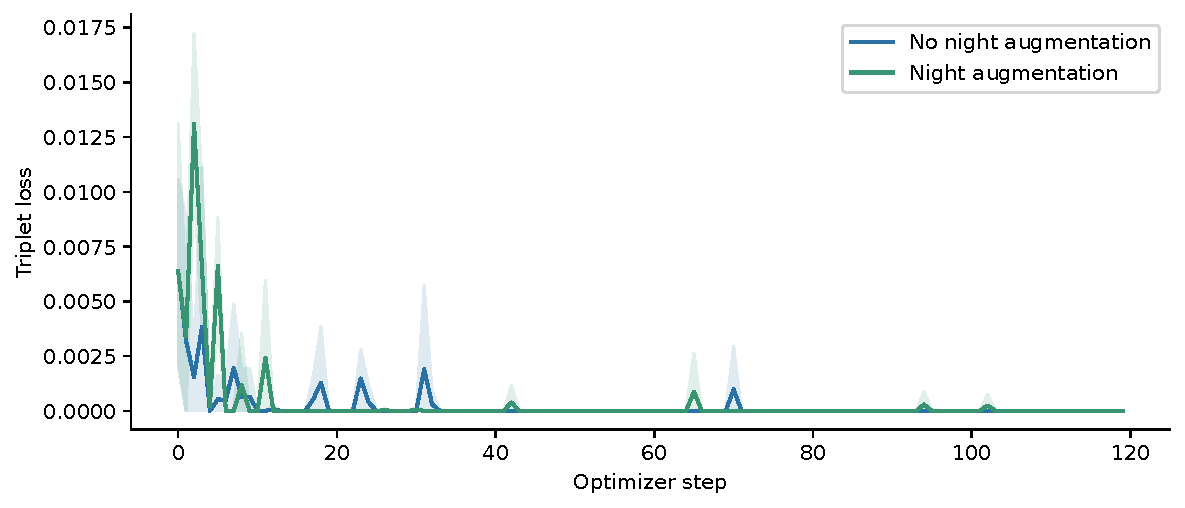
\includegraphics[width=\textwidth]{training_loss.pdf}
\caption{Actual triplet-loss traces from the executed frozen-backbone projection experiment. Curves average fixed training seeds and shaded regions show their observed range. Lower training loss is not a held-out retrieval result.}\label{fig:training-loss}
\end{figure}
\Cref{fig:training-loss} shows that the small head can optimise the selected training objective. That does not imply that its compressed embedding preserves all ranking information required by Tokyo or the held-out viewpoint sequences. The experiment changes both dimensionality and training distribution; those effects are not separately identified. A future study should compare an untrained fixed compression control and longer, geographically broader adaptation before attributing changes specifically to synthetic night pairs.
\fi

The reported intervals use only three fixed seeds and are therefore broad where the outcomes vary. Deterministic pretrained scores repeated across seed rows have zero seed variance, which does not mean zero data uncertainty. The table separates training randomness from the unmeasured variability of collecting different places. No best-seed checkpoint was selected for the deployment claim.

\section{Qualitative correspondences and overlays}
\begin{figure}[htbp]\centering
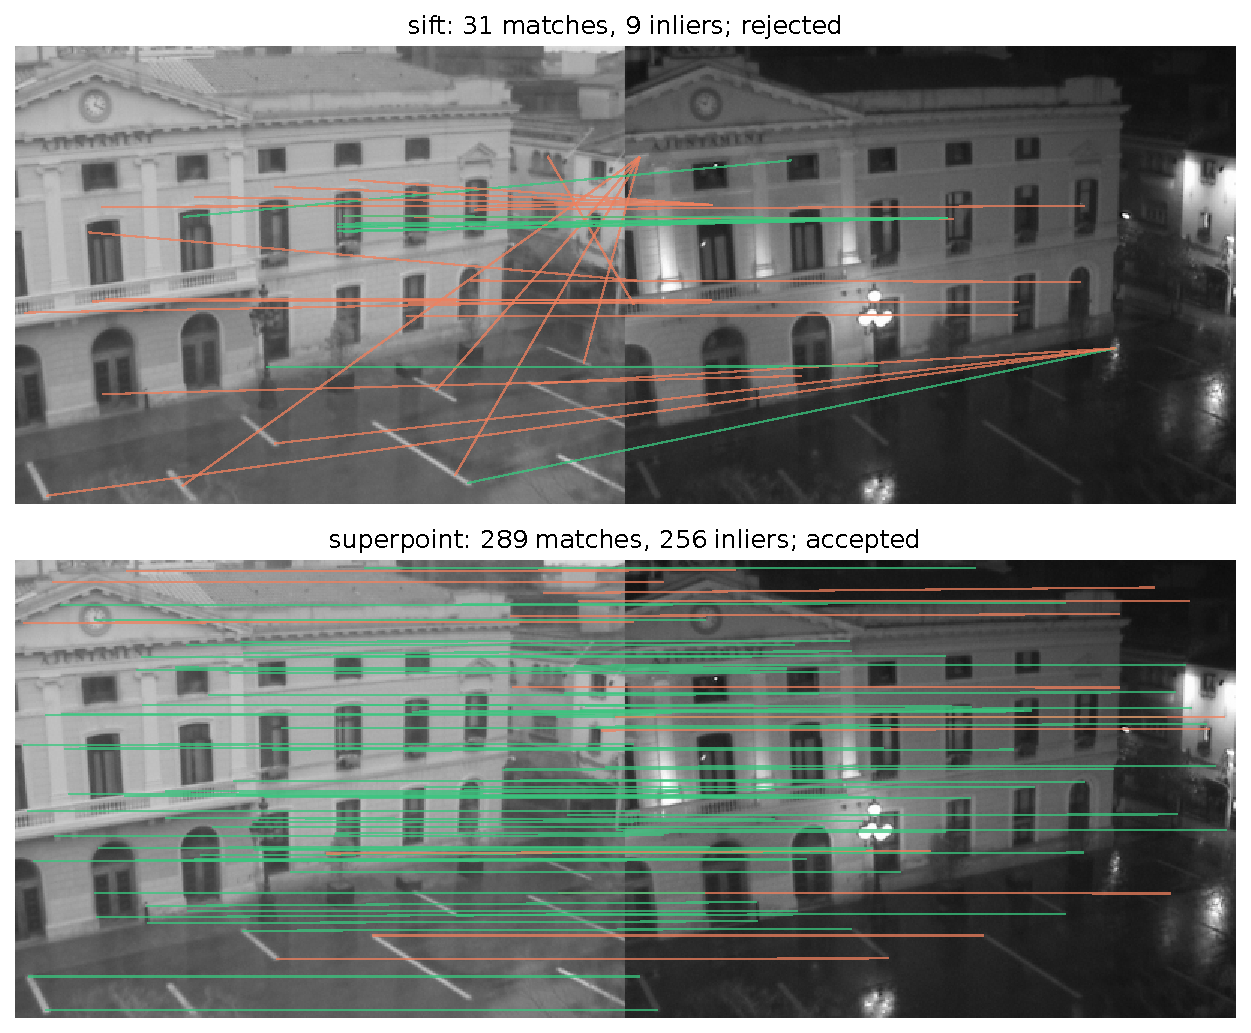
\includegraphics[width=\textwidth]{matches_hpatches_illumination.pdf}
\caption{Executed correspondence visualisation for the documented illumination example. At most eighty actual tentative correspondences are drawn per panel; green denotes the saved RANSAC inlier mask and orange denotes other tentative matches.}\label{fig:matches-illum}
\end{figure}
\Cref{fig:matches-illum} shows how the numerical support arises on a selected example. The displayed lines are a deterministic subset of actual correspondences, not an illustration invented independently of inference. Their colour reflects RANSAC compatibility, which should not be confused with an independent manual label for every match.

\begin{figure}[htbp]\centering
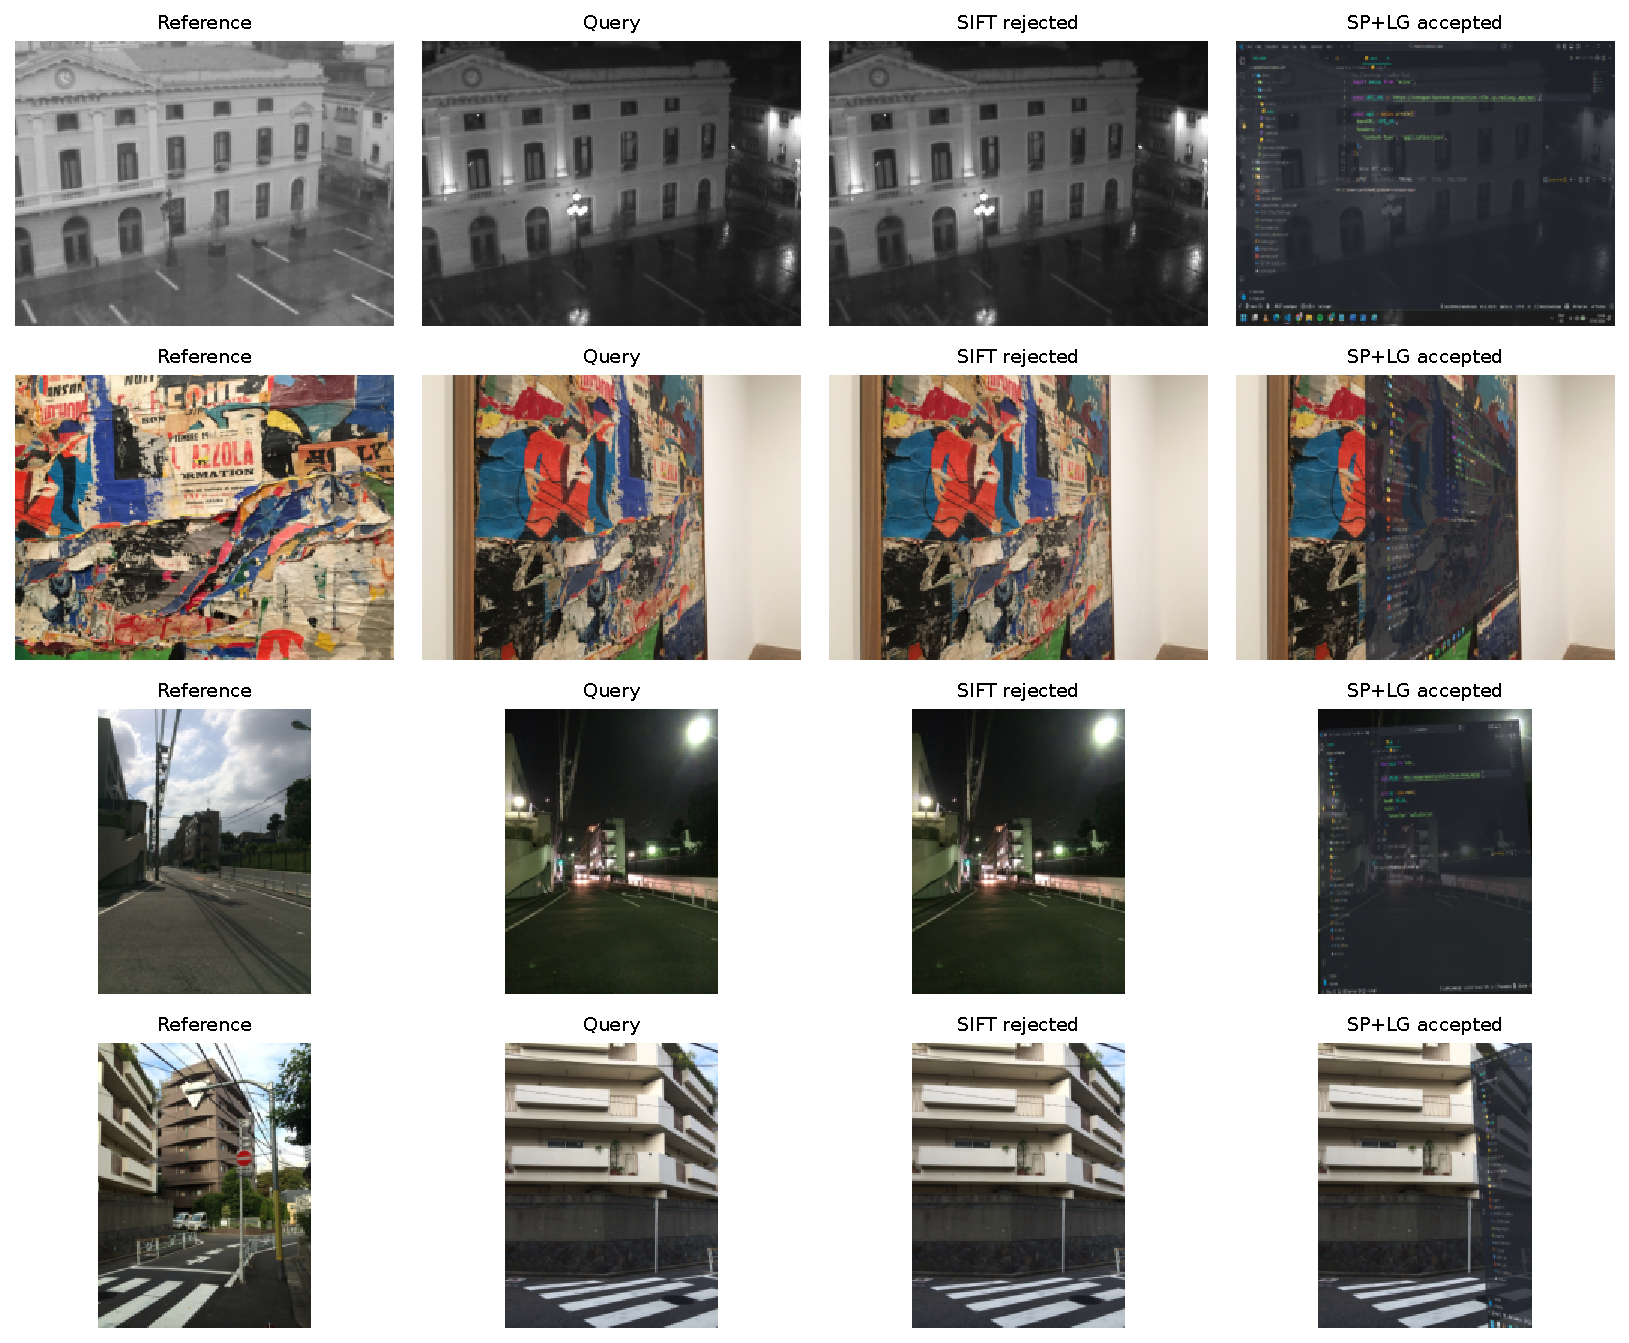
\includegraphics[width=\textwidth]{qualitative_overlays.pdf}
\caption{Saved-transform overlay examples across illumination, viewpoint and Tokyo protocols. Rejected geometry leaves the query unchanged. Accepted Tokyo overlays remain planar demonstrations without ground-truth pose or full-scene planarity.}\label{fig:overlays}
\end{figure}
\Cref{fig:overlays} links the geometry to the original application. An accepted map can support an attached image, and rejection remains visible rather than being replaced with a ground-truth or manually aligned overlay. A plausible street overlay is still not proof of correct depth, occlusion, or world-scale persistence. \ifFullReport Additional match visualisations and their selection rule appear in \cref{app:qualitative}.\fi

The demo uses real selected day and night photographs with generated small two-dimensional camera motion. It is explicitly labelled as generated motion rather than real temporal video captured in those conditions. Both complete pipelines execute on each generated query frame. The bundled source video is separately used for the original-script execution and CLI smoke test. These demonstrations establish implemented data flow and rendering, not high-frequency real-world tracking performance.

\section{Uncertainty and unavailable measurements}
\resultinput{confidence.tex}
\Cref{tab:confidence} prevents perfect observed rates from being read as certainty. The Wilson intervals remain finite-sample statements about the chosen site set under the stated approximation. Cluster-bootstrap intervals for HPatches are also retained in the generated statistics artifact. Neither procedure removes the selection bias of a small geographic subset or repairs missing calibration.

\resultinput{pose-unavailable.tex}
\Cref{tab:poses} records a requested but unmeasured result. No metric translation-and-rotation rates are inferred from GPS identities or homography corner errors. Likewise, there is no real seasonal benchmark result, phone power measurement or city-scale service cost. The report distinguishes these absences from actual negative results such as wrong accepted places or reduced retrieval after adaptation.

\section{Threats to validity}
\subsection{Internal validity}
The normalised local comparison shares preprocessing dimensions, feature budgets and geometry settings, but it cannot equalise the internal training data or detector semantics of pretrained models. Approximate descriptor search and floating-point kernels can introduce small run differences. Fixed seeds, exact model hashes and cached pair accounting reduce ambiguity, while the separate original-script runs avoid conflating the refactor with unchanged upstream behaviour.

Some evaluation stage timings were recorded while independent preparation tasks were also active. They are therefore treated as accounting diagnostics. The isolated complete-query profiles are the principal latency evidence. Even those profiles use a small fixed query selection and a warmed process, so they do not describe cold mobile startup or worst-case thermally constrained execution.

\subsection{Construct validity}
Inlier support is not ground-truth correspondence accuracy, accepted geometry is not true alignment, and place recognition is not metric localisation. The report reports those constructs separately. The planar corner metric itself measures extrapolation to the reference boundary, which may penalise a locally useful surface match. That is appropriate for a full-reference overlay but should be reconsidered for a smaller user-defined anchor region.

The custom Tokyo gallery changes the benchmark problem. Its perfect aligned cross-time results should be read alongside its viewpoint failures and small denominator. Synthetic night and fog labels describe transformations, not natural capture conditions. The proposed mobile architecture is not an implemented phone deployment. These boundaries are retained in captions and prose to prevent a demonstration from being used as evidence for a stronger construct.

\subsection{External validity}
The selected scenes, geographic region and reference directions do not cover the intended worldwide application. There are no measured seasonal transitions, construction changes, crowds, adversarial displays or long-term map revisions. A production gallery would include many more near-duplicate structures and unknown places. Extrapolating the measured false-acceptance rate or retrieval saturation to that setting would be unjustified.

\subsection{Statistical conclusion validity}
The sample is small and correlated. Three training seeds cannot characterise the full optimisation distribution, and a larger number of synthetic pixels does not create independent physical places. Intervals are presented with their grouping assumptions, not as proof of a universal method ranking. The conclusions emphasise supported direction and failure mechanisms rather than claiming statistical superiority across all deployment conditions.

\section{Implications for the research questions}
The measured evidence supports learned local matching for the selected illumination changes, while providing no uniform viewpoint advantage under the planar criterion. Global retrieval can retain aligned cross-time recognition with fewer local comparisons, but it limits success under the tested direction change. Geometry reduces indiscriminate acceptance yet still produces some wrong-place decisions. Short projection adaptation is not a reliable improvement here. The executed export establishes a practical descriptor-only deployment artifact, whose trade-offs are examined next.
